\documentclass[thesis.tex]{subfiles}
\begin{document}

\chapter{Concept}\label{chap:concept}

In this chapter, a detailed description of the chosen approach used to achieve the desired goal will be presented. Section~\ref{cpugpupartitioning} discusses the potential options for workload partitioning between the CPU and the GPU. Section \ref{porting} elucidates the steps and strategies necessary for porting the serial algorithm to CUDA. Section~\ref{dmmse} presents the idea of a custom memory allocator that is capable of recycling and reusing the DRAM allocations. Section~\ref{psdec} outlines the chosen strategy for generating large-scale power systems that can be easily partitioned. Section~\ref{consync} provides a description of the concurrency and synchronization techniques used for maximize compute-resource utilization. Section~\ref{merg} discusses a simple process of merging local states into global states. 

\section{CPU-GPU Workload Partitioning}\label{cpugpupartitioning}
Most CPU manufacturers enable programmers to utilize their own processor-specific BLAS and LAPACK implementations, e.g. Intel Math Kernel Library and AMD LibM. These libraries are optimized for accuracy and performance in comparison to the compiler-provided math functions. Hence in heterogeneous computing, there exists a possibility to exploit these libraries in conjunction with GPU. \\
As shown in Figure~\ref{fig:workpartition}, the host and the device are connected via a Peripheral Component Interconnect Express (PCIe) interface which offers high bandwidth communication between the device and the motherboard. If PCIe v3x16 (3rd Generation, with 16 lanes) is used, the maximum bandwidth available is 985 MB/s * 16 = 15.75 GB/s. Although this data-rate is very high, for large-scale general purpose heterogenous computations, this can be a potential bottleneck. 
\begin{figure}[H]
	\centering
	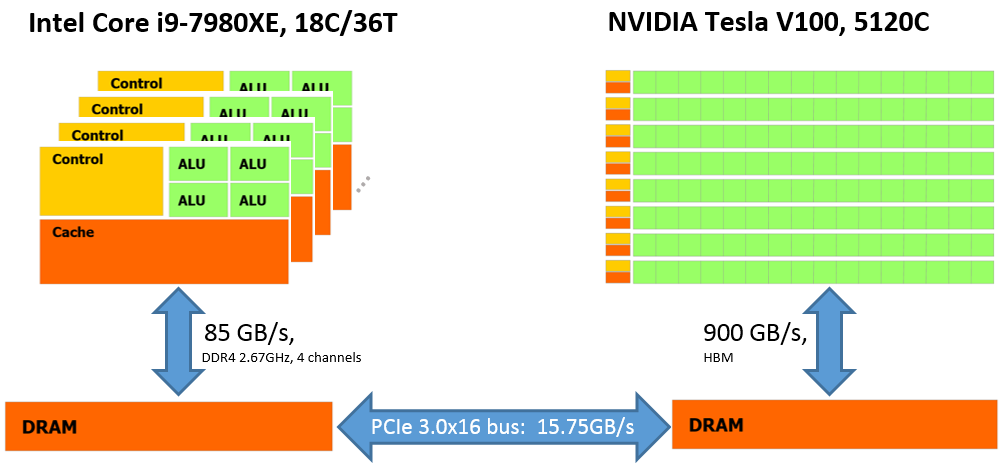
\includegraphics[scale=0.55]{workpartition}
	\caption{Bandwidths of various memory interfaces on modern CPU and GPU}
	\subcaption*{The major potential bottleneck in heterogeneous computing is the interface between the CPU and the GPU.}
	\label{fig:workpartition}
\end{figure}
During any GPU-accelerated computation including SE, there are two types of workloads:
\begin{enumerate}
	\item \textbf{Arithmetic Computations}:
	These tasks can run either on the host or on the device or in conjunction. If running in conjunction, this leads to better compute-resource utilization as the CPU is not waiting idle for the kernels launched asynchronously to complete. Instead, CPU can be assigned its own arithmetic workload which overlaps with GPU executions and therefore resulting in reduced processor-idle-states. 
	\item \textbf{Control Logic}:
	Control tasks are generally handled by the host. These include launching arithmetic computations via kernels to run on the GPU, data transfers to and from the device and performing certain checks. However, modern GPUs are capable of launching child-computations from parent computations as well as handling control logic.
\end{enumerate}
The following table~\ref{table:matOpsTar} shows the sample accelerations of various arithmetic operations on the GPU. The performance boost obtained without transferring the result to the CPU is always higher. This is because of the the transfer over PCIe is expensive.
{\renewcommand{\arraystretch}{1.2}%
\begin{table}[H]
	\begin{tabular}{|l|l|l|}
		\hline
		\multicolumn{1}{|c|}{\textbf{Targeted Matrix Operation}} & \multicolumn{1}{c|}{\textbf{\begin{tabular}[c]{@{}c@{}}Performance Boost\\ (without PCIe transfer)\end{tabular}}} & \multicolumn{1}{c|}{\textbf{\begin{tabular}[c]{@{}c@{}}Performance Boost\\ (with PCIe transfer)\end{tabular}}} \\ \hline
		Addition (10x10 matrices)                                & {\color[HTML]{CB0000} 0.01x}                                                                                      & {\color[HTML]{CB0000} 0.008x}                                                                                  \\ \hline
		Addition (100x100 matrices)                              & {\color[HTML]{CB0000} 0.1x}                                                                                       & {\color[HTML]{CB0000} 0.029x}                                                                                  \\ \hline
	\end{tabular}
	\begin{tabular}{|l|l|l|}
		\hline
		\multicolumn{1}{|c|}{\textbf{\begin{tabular}[c]{@{}c@{}}Targeted Matrix Operation\\ (5000x5000 matrices)\end{tabular}}} & \multicolumn{1}{c|}{\textbf{\begin{tabular}[c]{@{}c@{}}Performance Boost\\ (without PCIe transfer)\end{tabular}}} & \multicolumn{1}{c|}{\textbf{\begin{tabular}[c]{@{}c@{}}Performance Boost\\ (with PCIe transfer)\end{tabular}}} \\ \hline
		Addition                                                                                                                & {\color[HTML]{036400} 7.05x}                                                                                      & {\color[HTML]{CB0000} 0.42x}                                                                                   \\ \hline
		Subtraction                                                                                                             & {\color[HTML]{036400} 7.27x}                                                                                      & {\color[HTML]{CB0000} 0.42x}                                                                                   \\ \hline
		Multiplication                                                                                                          & {\color[HTML]{036400} 6.98x}                                                                                      & {\color[HTML]{CB0000} 0.41x}                                                                                   \\ \hline
		Division                                                                                                                & {\color[HTML]{036400} 7.28x}                                                                                      & {\color[HTML]{CB0000} 0.41x}                                                                                   \\ \hline
	\end{tabular}
	\caption{Speedups on GPU for various elementwise operations}
	\subcaption*{ Larger performance boost is better; Values larger than 1 indicate positive speedups.\\
		Hardware: Intel i5,  NVIDIA GTX 1070; \\
		Software: NumPy + Intel MKL, CUDA 9.}
	\label{table:matOpsTar}
\end{table}}

From these results, two conclusions can be drawn:
\begin{enumerate}
	\item Although there exists a possibility to run compute-intensive DLA arithmetics on CPU in conjunction with the GPU, the speedup on GPU is remarkably large. Hence, misassignment of large-scale compute-intensive workloads to the CPU just for greater resource utilization can produce degraded performance. 
	\item If used in conjunction, the data-transfer costs over PCIe significantly impacts the otherwise achievable boost, i.e. when results need not be transferred to the CPU. Therefore in case of a program running several operations on the GPU, the intermediate results must stay on the GPU until the final results have been computed and ready.
\end{enumerate}

The above conclusions are especially noteworthy since the matrices used in SE for large power systems like IEEE 118-bus can have dimensions in the upwards of 1000. Due to this, it can be safely assumed that moving all the arithmetic computations to the GPU is indispensable. \\
Once this appropriate CPU-GPU work partitioning is decided, the computational workload on GPU can be handled with or without further CPU intervention once the mandatory host-side initialization is complete. This is achieved through Dynamic Parallelism feature supported by modern NVIDIA GPUs which allows on-demand spawning of new kernels on the GPU dynamically, thereby making it no longer just a coprocessor. An explanation on these two approaches is described below:

\subsection{SE without Dynamic Parallelism}\label{sec:wodp}
As shown in Figure~\ref{fig:wodp}, at the end of every WLS iteration for SE, the maximum residual error $\delta$ is transferred to the host. If the error is greater than a predetermined constant, (i.e. if convergence criterion is not met) another iteration of WLS must be launched. Since the entire arithmetic workload is offloaded to the device, the responsibility of the CPU is limited to launching the CUDA kernels and evaluating whether the convergence criterion is met after every WLS iteration. \\
With this chosen technique of workload partitioning, the data transfers between the host and device is limited to the transfer of a double(or a float) value per iteration. 
\begin{figure}[H]
	\centering
	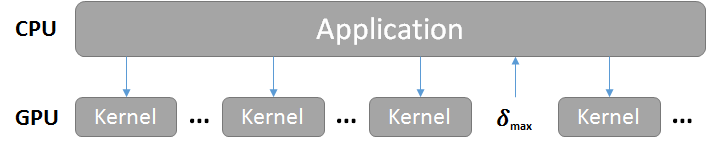
\includegraphics[scale=0.6]{wodp}
	\caption{High-level structure of conventional GPU-accelerated WLS-SE application}
	\label{fig:wodp}
\end{figure}

\subsection{SE with Dynamic Parallelism}\label{sec:wdp}
Dynamic Parallelism is introduced by NVIDIA in 2013 with the release of CUDA 5.0. Modern NVIDIA GPUs are capable of launching children workloads dynamically and this presents developers with an opportunity to reduce the dependence on the host (observed in conventional GPU-accelerated applications). This also means the per-iteration transfer previously necessary can be now handled within the GPU. 
\begin{figure}[H]
	\centering
	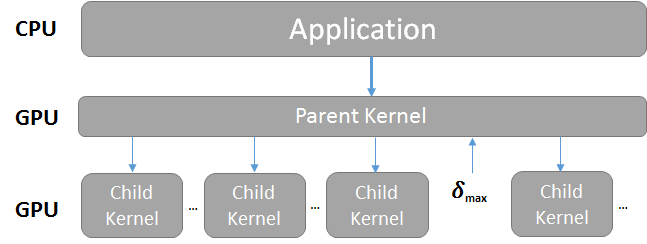
\includegraphics[scale=0.6]{wdp}
	\caption{High-level structure of DP WLS-SE Application}
	\label{fig:wdp}
\end{figure}

As seen above in Figure~\ref{fig:wdp}, the parent kernel launches multiple child kernels. The child kernel may themselves launch other kernels, resulting in a nested execution hierarchy with a permitted depth of 24 generations. However, this depth of the hierarchy is generally limited by available device resources.\\
Therefore, it can be assumed from the above discussion that WLS algorithm’s arithmetic computations as well as control logic can be offloaded to the GPU; thereby limiting the role of CPU to initialization. This approach keeps the invoking CPU thread on hold until the computation converges and the state vector is returned to the host for subsequent use.


\section{Porting Serial Algorithm to GPU}\label{porting}
GPU-accelerations are introduced to an existing application through Assess, Parallelize, Optimize, Deploy (APOD) design cycle. As shown in Figure~\ref{fig:apod}, it is a cyclical process through which programmers can incrementally identify hotspots within the application that can benefit from the porting. The produced accelerated counterparts are then subjected to further possible optimizations (e.g. cache usage, coalesced memory access etc.) and a faster version of the application is then deployed into production.\\
\begin{figure}[H]
	\centering
	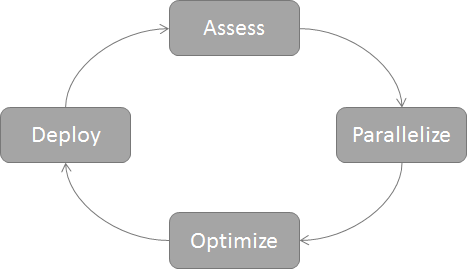
\includegraphics[scale=0.55]{apod}
	\caption{APOD Design Cycle}
	\label{fig:apod}
\end{figure}
In order to analyse the viability of decentralization of SE on GPU, the serial algorithm for SE must be ported to its programming platform. Apart from moving the arithmetic workload entirely to the device and reducing the data transfers to the bare minimum, attention must be paid to the fact that all matrix arithmetics on the GPU that require launching kernels come with certain overhead~\cite{kernelOverhead}. \\
For latency-critical applications, a large number of kernel-launches naturally implies a large overhead which may result in performance degradation. The following is a list showing overhead (amortized) for asynchronous empty CUDA kernel launches across some GPUs with different architectures:
\begin{itemize}
	\item Quadro K2100M: 0.0139ms
	\item GTX 1070: 0.003ms
	\item Tesla V100: 0.006ms
\end{itemize}
Taking this into consideration, it is important that the number of kernel launches be minimized. Alongside this, there are certain other guidelines during preparation of a data-parallel GPU-equivalent of the serial algorithm which are described as follows:
\subsection{High Level Guidelines adopted for GPU Migration}
\subsubsection{Recomputation Avoidance}
Throughout the algorithm, there are several instances of computations which are repetitive. An instance of such cases is shown below:\\
\begin{equation}\label{eq:repA}
\textbf{\textit{A}} = \textbf{\textit{X}}^{T}\textbf{\textit{Y}} + \textbf{\textit{P}}
\end{equation}
\begin{equation}\label{eq:repB}
\textbf{\textit{B}} = \textbf{\textit{X}}^{T}\textbf{\textit{Y}} + \textbf{\textit{Q}}
\end{equation}

In the operations \ref{eq:repA} and~\ref{eq:repB}, a component is identical in both the calculations. On CUDA, this will result launch of 6 kernels, i.e. 2 for transpose, 2 for dot products and 2 for additions. If left unoptimized, this shall result a transpose operation followed by a dot product for the same data twice. It is very important that such spots are located in the algorithm and fixed in the following manner:\\
%\begin{equation*}
%	\begin{array}{1}
%		\textbf{\textit{D}} = \textbf{\textit{X}}^{T}\textbf{\textit{Y}} \\
%		\textbf{\textit{A}} = \textbf{\textit{D}} + \textbf{\textit{P}}\\
%		\textbf{\textit{B}} = \textbf{\textit{D}} + \textbf{\textit{Q}}
%	\end{array}
%\end{equation*}
\begin{equation*}
	\textbf{\textit{D}} = \textbf{\textit{X}}^{T}\textbf{\textit{Y}}
\end{equation*}
\begin{equation*}
	\textbf{\textit{A}} = \textbf{\textit{D}} + \textbf{\textit{P}}
\end{equation*}
\begin{equation*}
	\textbf{\textit{B}} = \textbf{\textit{D}} + \textbf{\textit{Q}}
\end{equation*}

With recomputation avoidance, the total of kernel launches achieving the same results is now 4 and is achievable in lesser time. Specifically in WLS loop, many repeating computations yielding the same values should be precomputed and used wherever necessary. 
\subsubsection{Coalesced Global Memory Access}
In CUDA architecture, a warp is referred to as a collection of 32 threads that are woven together to execute in a lockstep. A warp once scheduled executes the same instruction on different data in Single Instruction Multiple Data (SIMD) fashion. As the device coalesces global memory access from threads of a warp into as few memory transactions as possible to minimize memory latency, attention must be paid to analyse the memory access patterns in use. Each DRAM memory load transaction may be of 32 byte granularity or of 128 bytes with L1 cache enabled. Likewise, each memory store transaction is of 32 bytes.\\
When a memory request cannot be serviced in a single transaction, multiple such transactions must be launched causing increased memory latency. This performance may further be adversely impacted when the access patterns of a kernel is either misaligned or strided. \\\\
In Figure \ref{fig:coag}, the access pattern is aligned since the starting address of the memory is an even multiple of 128 bytes. 
It is called coalesced since each thread reads from a contiguous memory location. Figure~\ref{fig:coag} displays an ideal case for an ideal memory access pattern. Each thread is reading a byte values from each memory location. Irrespective of whether global memory or L1 cache is used to perform this load, the starting address is an even multiple of 32 as well as 128. Hence, this would result in 100\% memory bus utilization and zero wasted values.

\begin{figure}[H]
	\centering
	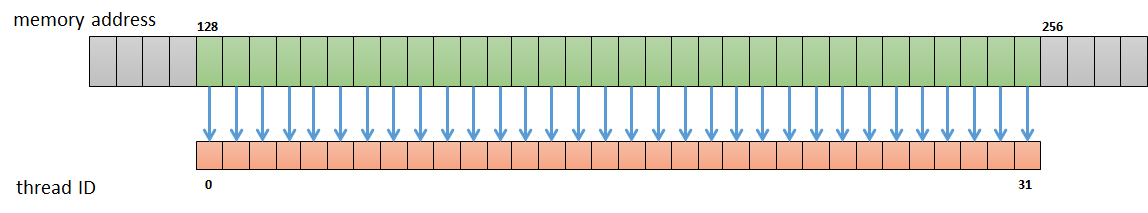
\includegraphics[scale=0.5]{coag}
	\caption{Aligned and coalesced memory access}
	\label{fig:coag}
\end{figure}

\subsection{Prevention of Shared Memory Bank Conflicts}
The on-chip location of shared memory makes it roughly 100 times faster than global memory. Shared memory is split in equally sized memory banks to enable high-bandwidth concurrent accesses. When multiple threads of a block in a warp access the same address in shared memory, it results in a multicast. However, when multiple threads try to access different addresses from the same memory bank, it results in the memory requests getting serialized thereby adversely impacting the bandwidth. 
This usually occurs when working with matrices of double datatype and its prevention is very crucial. 


\subsection{Prevention of Warp Divergence}
Since threads are executed in a group of 32, a variation in the execution trajectories of the threads results in the warp collectively not executing the same instructions. The most common programming construct that leads to a warp divergence is the branching due to conditionals as in an if-then-else statement or a switch statement. Such branching leads to a part of the warp getting masked off while the threads with true conditions are active. Since the branches get executed serially, this breaks the SIMT fashion of CUDA and results in serialized execution. Such branching logics must be avoided to prevent performance degradation.

\subsection{Utilization of Official GPU Libraries}
GPU computing is often supported by the manufacturers through the release and maintenance of official and affiliate libraries. NVIDIA provides official BLAS and quasi-LAPACK implementations, namely cuBLAS and cuSOLVER on the top of CUDA runtime. These GPU libraries are a part of CUDA installation and the optimized nature of these libraries makes it possible to save development time and gain performance. It is therefore highly recommended to make use of these libraries wherever possible.



\section{Device Memory Management For Large-Scale SE Computation}\label{dmmse}
The amount of memory on a host can be extended based on user requirements. Most modern workstations have DDR3 or DDR4 RAMs in the range of 16-32 GB. However, a dedicated GPU has a non-upgradable V-RAM, e.g. 32-bit GDDR5 or more recently, 1024-bit HBM RAM. The rise of use in HBM for reduced chip complexity and improved power consumption has made it impossible to potential tinkering/desoldering by enthusiasts as the memory is etched directly on the package substrate. \\
For a DLA GPU computation running for a finite time and iterations, the memory requirements to hold variables can be predicted. On the contrary, for processing tasks with unknown number of iterations, memory consumption is also unknown. Considering the limited size of DRAM available, efficient memory management is mandatory.\\
In addition to the above, the allocation and deallocation of device memory blocks can be expensive and the costs increase with the size of memory requested~\cite{allocationOverhead}. Although allocations cannot be avoided, the deallocations must not be started until the end of the execution.\\\\
Hence, to deal with the limited DRAM constraint, some of the strategies are discussed below:
\begin{enumerate}
	\item Every arithmetic calculation present in SE’s WLS iteration is defined as a ‘step’. Each step consists of certain intermediate computation components followed by the result. The memory consumed by these intermediate components must be immediately released after the result for the concerned step is computed. For example,\\
	\begin{equation*}
		g(x^{k}) = -H^{T}(x^{k}).R^{-1}.(z-h(x^{k}))
	\end{equation*}
	In the example step above, the final results is stored in matrix $g(x^{k})$ and these values is necessary throughout the given iteration. The matrix $g(x^{k})$ can be placed ‘\textbf{on hold}’ for the rest of the iteration. However, the intermediate operations such as the dot products and the inverse have memory allocations (MA) occupied that must be released for the subsequent steps.
	\item At the end of each iteration, if the convergence criterion is not met, all the matrices placed \textbf{on hold} in the current iteration must be released. With this action, the memory needed for subsequent iteration is released thereby availing resources for next batch of calculations.
	\item The new, in-use and released MAs can be placed in multiple pools based on their status in the computation. In WLS algorithm, the MAs can be placed in the following pools:
		\begin{enumerate}
			\item \underline{Do-Not-Disturb (DND) Pool}: 	
				This pool is used to hold values that should not be altered and/or freed throughout the execution of the program. The MAs in this pool are not released until the end of the execution. For example, measurement matrix, grid topology etc.
			\item \underline{Per-Iteration On-Hold Pool}:
				As the name suggests, this pool is used for holding MAs with values crucial for the given iteration of the WLS algorithm. This pool is flushed at the end of each iteration following which the contained MAs are sent to the Available Pool.
			\item \underline{Intermediate-use Pool}: 
				The MAs that get used for intermediate computations for every step of WLS algorithm are held in this pool. This pool requires frequent flushing so as to release the MAs back to the Available Pool. This act of flushing waste MAs makes them fit for reuse in subsequent steps.
			\item \underline{Available Pool}: 
				This consists of MAs that are available for use. These may include newly allocated or previously flushed MAs.
			
			\item \underline{Unallocated DRAM}:
				This is the free DRAM that is still available for allocation. With every allocation made, the amount of memory available in this pool decreases.
		\end{enumerate}
\end{enumerate}

The layout of an MA-pool is shown below in Figure \ref{fig:mapool}:

\begin{figure}[H]
	\begin{subfigure}{.4\textwidth}
		\centering
		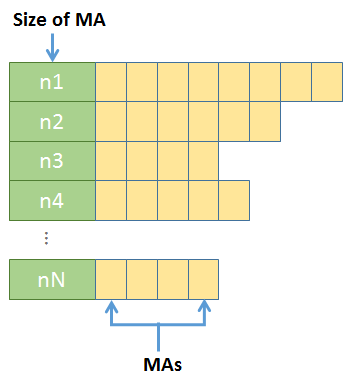
\includegraphics[width=.6\linewidth]{mapool}
		\caption{Memory allocation pool containing device pointers of various sizes}
		\label{fig:mapool}
	\end{subfigure}%
	\begin{subfigure}{.7\textwidth}
		\centering
		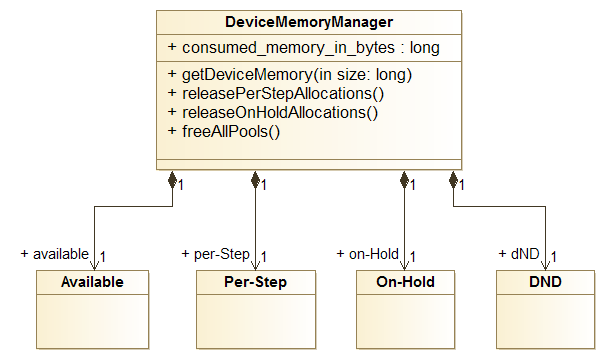
\includegraphics[width=.8\linewidth]{dmm}
		\caption{Class Diagram of Device Memory Manager}
		\label{fig:dmm}
	\end{subfigure}
	\caption{Design of Device Memory Manager}
	\label{fig:mapooldmm}
\end{figure}

This layout in Figure \ref{fig:mapool} can be realized using Map data-structure. Effectively, these pools hold arrays (or stacks) of equally-sized MAs as a dictionary, with the sizes of these MAs being the keys. 
Using the above 3 strategies of releasing intermediate and on-hold MAs and organizing them in various pools, a custom device memory manager (DMM) can be created that is capable of both creating new MAs and recycling the not-in-use existing ones. For every new MA request, a size is passed to the DMM. If the stack for the given size is empty, the DMM creates new MA. Otherwise, a pre-existing MA is returned. The structure of this memory manager is shown in the Figure \ref{fig:dmm}.

\section{Power System Decentralization}\label{psdec}
Since a power system is in essence an undirected graph comprising vertices(busses) and edges(lines), graph partitioning techniques can be used to distribute or decentralize a large global WLS SE problem into N smaller subproblems that can be solved individually. This shall produce increase in computational speed since the complexity of the original SE problem is reduced. The reduction of complexity is primarily due to the reduction in the order of various matrices necessary for SE. The partitions or sectors obtained from as a result of partitioning must have the qualities (discussed in \ref{ddec}) as follows:
\begin{enumerate}
	\item The partitions must be roughly balanced, i.e. the partitions must have almost equal population of busses.
	\item The partitions should have minimum possible number of connection between any two given sectors.
	\item The busses in each partition are contiguous, i.e. there does not exist an entirely disconnected bus in any partition. This ensures the observability of each partition~\cite{Xiong}.
	\item This implementation assumes an overlapping vertex (bus) containing a PMU on the edge connecting the vertex to the subsequent grid. 
\end{enumerate}

Figure~\ref{fig:part118} is an illustration of how IEEE 118-bus system would look like after partitioning based on the aforementioned qualities.
\begin{figure}[H]
	\centering
	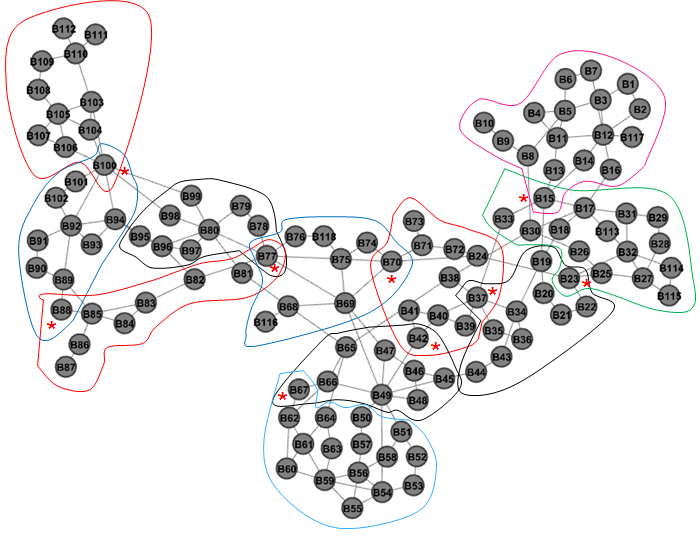
\includegraphics[scale=0.7]{part118}
	\caption{A well-partitioned IEEE 118-bus power system}
	\subcaption*{The partitioning satisfies all of the conditions above. The asterisk(*) indicates the presence of a PMU on the overlapping nodes.}
	\label{fig:part118}
\end{figure}

Graph partitioning problems are well known to be NP-hard. In order to partition grids that are 10 times (or more) larger than the IEEE 118-bus system, the potentially optimal solutions are typically obtained by using polynomial-time heuristics and approximation algorithms. Another alternative would be to construct larger grids through connected replication. Both of these approaches are described below:

\subsection{Automated Graph Partitioning}
Small partitioning problems with certain desirable properties can be solved by hand. However, for larger grids, this task can be cumbersome. Hence, there arises the need to partition graphs automatically. A variety of graph partitioning tool-boxes exist that can quickly compute the partitions. A possible solution could be the use of METIS from Section \ref{ddec} which is a set of serial graph partitioning programs based on multi-level recursive bisection and k-way partitioning schemes. METIS produces an assignment list that maps busses to different partitions. Using this result, the new topology data and relevant subsets of measurements for each sector can be computed.

\subsection{Innately Partitioned Grid}\label{subsec:innately}
In order to evaluate decentralized SE, large-scale sample grids must be prepared. Instead of subjecting several large standard IEEE grids to automatic partitioning, large-scale grids can be produced by duplication of relatively small IEEE grid followed by appropriate number of interconnections among the duplicates. Such grid chosen for duplication can be referred to as building-blocks. Figure \ref{fig:14bus} shows how 3 small IEEE 14-bus power systems can be connected to produce a larger 42-bus system.
\begin{figure}[H]
	\centering
	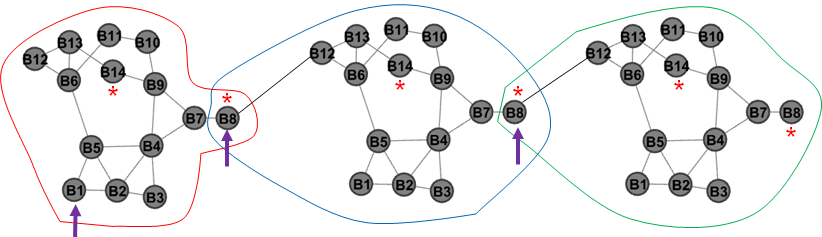
\includegraphics[scale=0.6]{14bus}
	\caption{Construction of large grid using IEEE 14-bus power system}
	\subcaption*{The overlapping partitions share a bus marked by an asterisk. The asterisk(*) indicates the presence of PMU. The arrows indicate the location of slack busses upon partitioning.}
	\label{fig:14bus}
\end{figure}

Although in practice, power systems are not constructed in this manner, such duplication technique may be used to construct large-scale power systems for evaluation purposes~\cite{KarimipourAcc}. However, the large-scale grids in question must be built using building block grids of sizes that benefit from acceleration through GPU-enabled SE.\\

When partitioning is required, each of the building-blocks can be readily considered as sectors alongside an overlapping bus from the preceding sector. In the previously constructed 42-bus system, there exists a slack bus where the phase is considered to be 0. However, upon partitioning, each sector contains its individual slack bus as seen in Figure~\ref{fig:14bus}. Considering overlapping busses for subsequent sectors following the first sector as the slack busses allows for easy communication of values and eventual merger of individual sector-states to obtain global states.

\section{Concurrency and Synchronization}\label{consync}
A large power system after decomposition (from Section~\ref{psdec}) into N smaller subproblems can be solved in separation from one another. If all the subproblems are solved sequentially, the total time required would be the summation of the time required for each subproblem’s solution, i.e.
\begin{equation*}
t = \sum_{i=1}^{N}t_{i}
\end{equation*}
One of the cornerstones of heterogeneous computing is to efficiently use all compute-resources in a given system. By the virtue of concurrency or multithreading, idle times on our multicore-processors and manycore-coprocessors can be reduced resulting in overall higher utilization. However, the CPU and the GPU platforms manage concurrencies differently. If the concurrencies are correctly applied, considerable performance boost can be achieved. That is, the total time taken is the time taken by the longest running subproblem as shown below:
\begin{equation*}
t = max(t_{1}, ... , t_{N})
\end{equation*}
With respect to Decentralized SE on GPU, the relevant concurrencies and necessary synchronization techniques are discussed below:
\subsection{Host-side Concurrency }
After the grid sectorization is complete, each sector may be subjected to separate SE computations as shown in Figure~\ref{fig:hscon}. Although in most favorable power flow situations, decentralized SEs executed sequentially provides speedups compared to the centralized approach, it can yet benefit further from concurrency. Irrespective of whether Dynamic Parallelism is used or not, each sector requires its independent initializations and solution. Considering CPU’s specialization in task-level parallelism, each sector can be assigned to a CPU thread. The thread is responsible for necessary data-transfers to/from the GPU, control flow and launching kernels. The responsibility however would be limited to initialization only in case DP is used.
\begin{figure}[H]
	\centering
	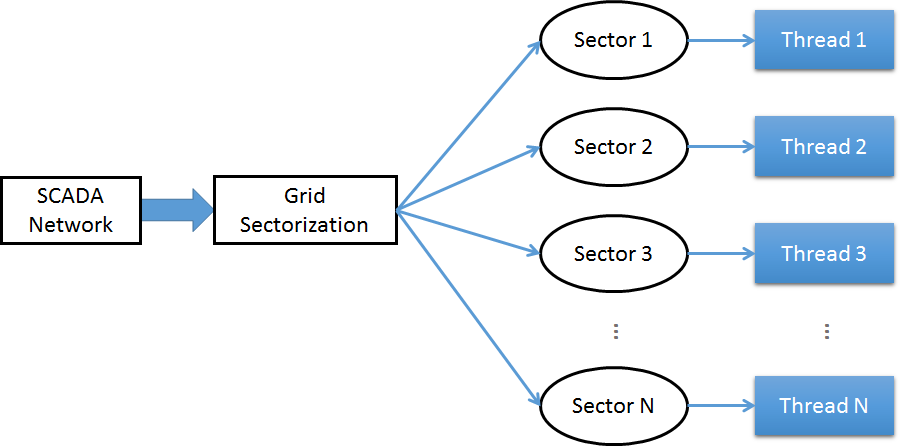
\includegraphics[scale=0.45]{hscon}
	\caption{Assignment of decentralized power system’s sectors to CPU threads.}
	\label{fig:hscon}
\end{figure}

Such assignment is due to the independent nature of each sector’s SE computations. Each thread is responsible for its own device memory management. 

\subsection{Device Concurrency}
In contrast to the host, higher resource utilization on the GPU can be achieved by managing concurrency on hardware work-pipelines (aka CUDA streams). A stream is a sequence of asynchronous commands that executes strictly in order. In CUDA, there are 2 types of streams:
\begin{enumerate}
	\item \underline{NULL stream}: It is the implicitly declared stream that exists by default.
	\item \underline{non-NULL streams}: These are explicitly declared streams defined by the user.
\end{enumerate}
When no stream is explicitly specified, all the commands get queued up in the NULL stream. On the other hand, a multithreaded host application seeking to benefit from concurrency offered by NVIDIA GPUs can launch the commands from each host thread on its private non-NULL streams. All the commands launched by a given thread in its respective stream undergo guaranteed in-issue-order execution. Similarly, commands issued by multiple threads on their respective streams undergo concurrent execution as shown in the Figure \ref{fig:dcon} below:

\begin{figure}[H]
	\centering
	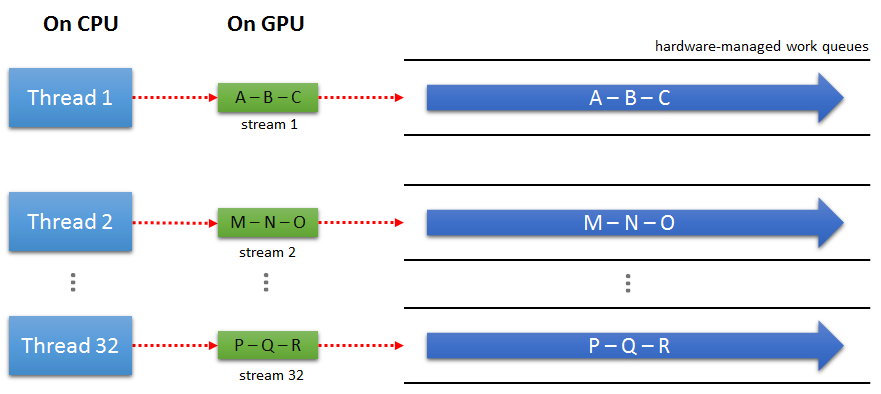
\includegraphics[scale=0.55]{dcon}
	\caption{Assignment of a non-NULL CUDA stream to each host thread}
	\label{fig:dcon}
\end{figure}

Although old GPUs like Fermi had only a single hardware work-queue resulting in multiplexed streams, modern NVIDIA GPUs come equipped with Hyper-Q technology which enables multiple CPU threads or processes to launch work on the same GPU simultaneously across multiple hardware work-queues(up to 32 concurrent streams); thereby resulting in increased utilization, enhanced performance and reduced energy consumption~\cite{Luley}. \\

As can be seen in Figure \ref{fig:dcon}, N threads are assigned to N non-NULL streams. This is especially suitable to build further on the sector-to-thread assignment from Figure \ref{fig:hscon}.\\
However, an issue associated with non-NULL streams is the need for explicit synchronization. This is due to the fact that only asynchronous CUDA commands can be launched on such streams. The need for such synchronization and the possible approaches are discussed below:

\subsubsection{GPU Synchronization for SE without Dynamic Parallelism}
In SE application not exploiting DP and launching CUDA commands on a non-NULL stream, the maximum residual error $\delta_{max}$ for each WLS iteration can be safely fetched to the host only after all preceding asynchronous operations have finished. The host thread must block until the concerned stream executions are over. From Figure \ref{fig:dcon}, since each CPU thread is bound to a GPU stream, the thread must create a synchronization barrier per iteration for  $\delta_{max}$ extraction. \\In CUDA, this is possible by calling \inlinecode{C}{cudaStreamSynchronize(stream)} function.


\subsubsection{GPU Synchronization for SE with Dynamic Parallelism}
In this case, the execution control is with the device. Assuming separate parent kernels are launched for each sector, with each parent kernel assigned to a non-NULL stream, it is again necessary to synchronize the stream to obtain per-iteration WLS maximum residual error $\delta_{max}$. However, CUDA Device Runtime does not support \inlinecode{C}{cudaStreamSynchronize(stream)} for per-stream synchronization. According to NVIDIA, ‘the only way to synchronize today is to wait for all work launched by a given thread to finish by calling \inlinecode{C}{cudaDeviceSynchronize()}’. This function waits for completion of all the child kernels previously launched by the parent kernel from which it has been called.

\section{Merger of State Vectors}\label{merg}
When each host thread has received its respective state vector, a merge operation is launched to obtain the global states. This is achieved by a simplified approach of adjusting the phases across the chain of sectors. In Figure \ref{fig:merger}, the overlapping node between any two given sectors is marked by the same color. Since the computations are performed considering the overlapping nodes as slack busses, the phase from the preceding sectors can be added to the slack of the following bus to obtain global angles. The voltages however are not subjected to any adjustment.
\begin{figure}[H]
	\centering
	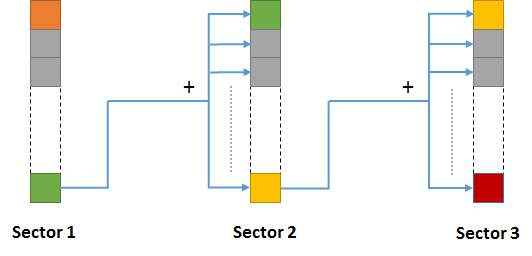
\includegraphics[scale=0.75]{merger}
	\caption{Merging of phase angles across sectors for obtaining global states}
	\subcaption*{Differences in phases of an overlapping node is used to adjust phases across the subsequent sector}
	\label{fig:merger}
\end{figure}
Another approach to merger of state vectors is a linear state estimation~\cite{Richter2} of individual sectors' state vectors in order to obtain the global states.



\chapter{Implementation}\label{chap:implementation}
This chapter presents the implementation details based on the ideas and concepts mentioned in Chapter~\ref{chap:concept}. Section~\ref{sec:hardware} describes the hardware and software setups. Section \ref{sec:accse} illustrates the 2 possible work-division techniques and related limitations. Section \ref{sec:portimpl} outlines the approaches used for porting serial operations to CUDA. Section \ref{sec:classdiagram} presents the application schematics and Section \ref{sec:integrationimpl} discusses the decentralized SE using developed SE application.

\section{Hardware and Software Setup}\label{sec:hardware}
The GPUs used for this implementation are Geforce GTX 1070 and Tesla V100 from NVIDIA. GTX 1070 is a generally-available GPU predominantly used for computer games whereas Tesla V100 is the current most advanced data-center GPU targeted at high-performance computing (HPC).
The detailed specifications of the graphics cards are listed below in table~\ref{table:harSofSetup}:
{\renewcommand{\arraystretch}{1.1}%
\begin{table}[H]
	\begin{tabular}{|l|l|l|}
		\hline
		\multicolumn{1}{|c|}{\textbf{Hardware}}                                             & \multicolumn{1}{c|}{\textbf{Geforce GTX 1070}}                                            & \multicolumn{1}{c|}{\textbf{Tesla V100}}                                              \\ \hline
		{\color[HTML]{000000} \begin{tabular}[c]{@{}l@{}}Compute\\ Capability\end{tabular}} & {\color[HTML]{000000} 6.1}                                                                & {\color[HTML]{000000} 7.0}                                                             \\ \hline
		{\color[HTML]{000000} CUDA Cores}                                                   & {\color[HTML]{000000} 1920}                                                               & {\color[HTML]{000000} 5120}                                                            \\ \hline
		{\color[HTML]{000000} \begin{tabular}[c]{@{}l@{}}Max\\ Clock Rate\end{tabular}}     & {\color[HTML]{000000} \begin{tabular}[c]{@{}l@{}}1.72 GHz\end{tabular}}                 & {\color[HTML]{000000} \begin{tabular}[c]{@{}l@{}}1.53 GHz\end{tabular}}              \\ \hline
		{\color[HTML]{000000} VRAM}                                                         & {\color[HTML]{000000} \begin{tabular}[c]{@{}l@{}}8 GB, GDDR5\end{tabular}}              & {\color[HTML]{000000} \begin{tabular}[c]{@{}l@{}}16 GB, HBM2\end{tabular}}           \\ \hline
		\begin{tabular}[c]{@{}l@{}}Memory\\ Bandwidth\end{tabular}                          & \begin{tabular}[c]{@{}l@{}}256 GB/s\end{tabular}                                        & \begin{tabular}[c]{@{}l@{}}900 GB/s\end{tabular}                                     \\ \hline
		\begin{tabular}[c]{@{}l@{}}SM\\ Count\end{tabular}                                  & 15                                                                                        & 80                                                                                     \\ \hline
		PCIe                                                                                & 3.0                                                                                       & 3.0                                                                                    \\ \hline
		\begin{tabular}[c]{@{}l@{}}Peak\\ FP32 Throughput\end{tabular}                      & \begin{tabular}[c]{@{}l@{}}6.4 TFLOP/s\end{tabular}                                     & \begin{tabular}[c]{@{}l@{}}14 TFLOP/s\end{tabular}                                   \\ \hline
		\begin{tabular}[c]{@{}l@{}}Peak\\ FP64 Throughput\end{tabular}                      & \begin{tabular}[c]{@{}l@{}}0.2 TFLOP/s\end{tabular}                                     & \begin{tabular}[c]{@{}l@{}}7 TFLOP/s\end{tabular}                                    \\ \hline
		\begin{tabular}[c]{@{}l@{}}CPU\\ RAM\end{tabular}                                   & \begin{tabular}[c]{@{}l@{}}Intel Core i5 (3.8 GHz, 4 CPUs)\\ 16 GB\end{tabular} & \begin{tabular}[c]{@{}l@{}}Intel Xeon (2 GHz, 8 CPUs)\\ 32 GB\end{tabular} \\ \hline
		\begin{tabular}[c]{@{}l@{}}Operating System \\ IDE\end{tabular}                     & \begin{tabular}[c]{@{}l@{}}Windows 10 \\ Visual Studio 2015\end{tabular}                  & \begin{tabular}[c]{@{}l@{}}Windows Server 2012 r2 \\ Visual Studio 2015\end{tabular}   \\ \hline
	\end{tabular}
	\caption{GPU test environment}
	\label{table:harSofSetup}
\end{table}}
Since the compute-capabilities of the used GPUs are 6.1 and 7.0, the compilation can be expedited by removing code generation for other compute-capabilities.\\
CUDA Runtime API can be accessed through a range of popular programming languages. It is usually a choice left to the programmer, available time for development and performance requirements. Some of the available options are listed below:
\begin{itemize}
	\item \textbf{CUDA Toolkit} : Official comprehensive environment for creating GPU-accelerated applications
	\item \textbf{CUDA FORTRAN}: Language solution developed in collaboration with The Portland Group.
	\item \textbf{PyCUDA}: MIT-licensed easy Pythonic access developed by Andreas Kloeckner
	\item \textbf{jCUDA}: MIT-licensed Java bindings for CUDA
	\item \textbf{Alea GPU}: Professional and cross-platform GPU software development environment (SDE) for .NET and Mono.
\end{itemize}
Although there exists many options as listed, CUDA Toolkit is the SDE of choice for this implementation. This is due to the following 3 reasons:
\begin{enumerate}
	\item The official status of the SDE makes it more robust and well-maintained.
	\item CUDA Toolkit API is based on C/C++. The compiled nature of these languages delivers high performance.
	\item Availability of official profiling and debugging tools like Visual Profiler or Nsight.
\end{enumerate}

\section{GPU-accelerated SE}\label{sec:accse}
\subsection{Base Serial SE Algorithm}\label{sec:bsealgo}
The SE algorithm used in this implementation is based on the fast terminal-modeled WLS SE given by Richter et al~\cite{Richter}. Terminal-modeling of power systems enables incorporation of measurements from synchrophasors meanwhile maintaining high computational efficiency. Instead of describing a power system using an adjacency matrix between the busses, terminal modeling enables description of the power grid using an adjacency matrix between busses and adjoining terminals in which each consecutive pair of terminals represent an edge between busses. This matrix is known as Node-terminal-incidence matrix ($\textbf{\textit{K}}_{KT}$). Similarly, the terminal admittance matrix describing the relation between the terminal voltages and current is given by $\textbf{\textit{Y}}_{T}$.\\
According to Richter et al~\cite{Richter}, measurement function $\textbf{\textit{h}}(\textbf{\textit{x}})$ and measurement Jacobian $\textbf{\textit{H}}(\textbf{\textit{x}})$ can be computed using the following 3 matrices:
\begin{enumerate}
	\item Measurement vector, $\textbf{\textit{z}}$
	\item Node-terminal-incidence matrix, $\textbf{\textit{K}}_{KT}$ 
	\item Terminal-admittance matrix, $\textbf{\textit{Y}}_{T}$  
\end{enumerate}

\begin{figure}[H]
	\centering
	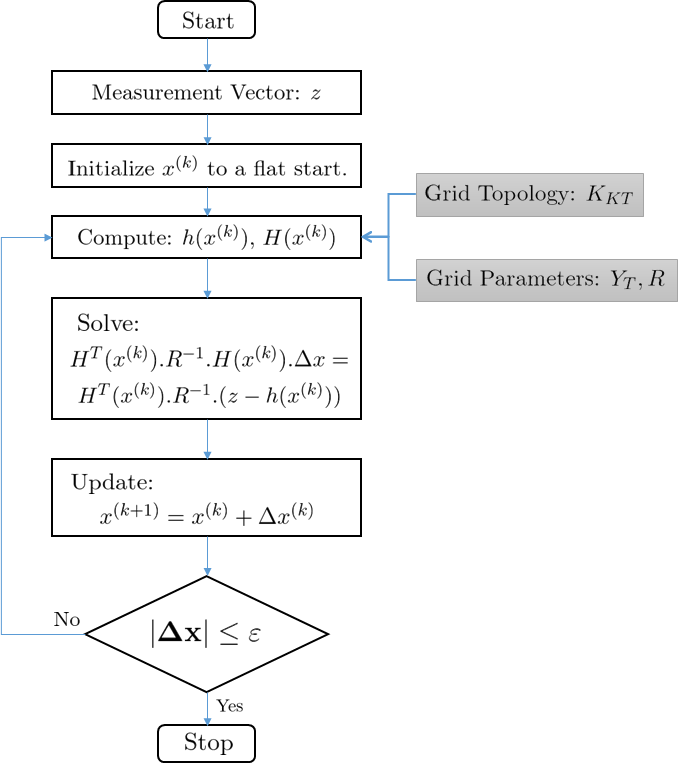
\includegraphics[scale=0.6]{tmwlsoverview}
	\caption{Overview of Terminal-modeled WLS SE}
	\label{fig:tmwlsoverview}
\end{figure}

As seen in the Figure \ref{fig:tmwlsoverview}, once $\textbf{\textit{h}}(\textbf{\textit{x}})$ and $\textbf{\textit{H}}(\textbf{\textit{x}})$ are computed with the help of grid topology and parameters, the $\Delta \textbf{\textit{x}}$ is obtained after solving the linear system of equations. However, the loop continues until the $\Delta \textbf{\textit{x}}$ is greater than a predetermined constant. 

\subsection{SE using CUDA}
As discussed in Section \ref{sec:wodp} and \ref{sec:wdp}, the base serial SE algorithm (described in Section~\ref{sec:bsealgo}) can be ported to CUDA and executed with or without Dynamic Parallelism. The major difference between these 2 implementations is the extent to which CPU interferes in the computations. The flowcharts in Figure~\ref{fig:cudasewodp} and Figure~\ref{fig:cudasewdp} illustrate the working mechanism of both the approaches.\\\\

\begin{figure}[H]
	\centering
	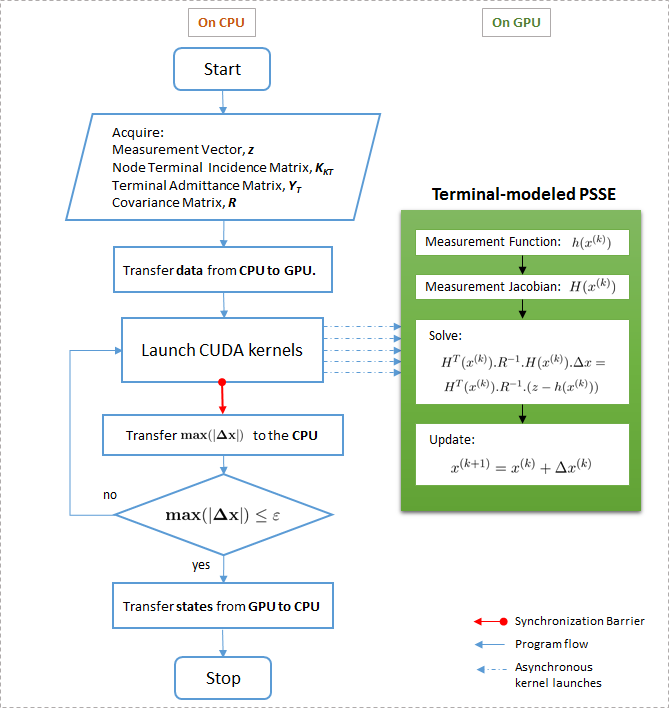
\includegraphics[scale=0.85]{cudasewodp}
	\caption{Ported SE using CUDA, without Dynamic Parallelism}
	\label{fig:cudasewodp}
\end{figure}

As shown in Figure~\ref{fig:cudasewodp}, the control for launching every iteration of WLS on the GPU is based on the evaluation of the convergence criterion handled by the host. The time taken for the transfer of $max|\Delta \textbf{\textit{x}}|$ to the CPU is about 13-15ns for both single and double precisions respectively. This transfer time can be entirely eliminated using Dynamic Parallelism as shown in Figure~\ref{fig:cudasewdp}.

\begin{figure}[H]
	\centering
	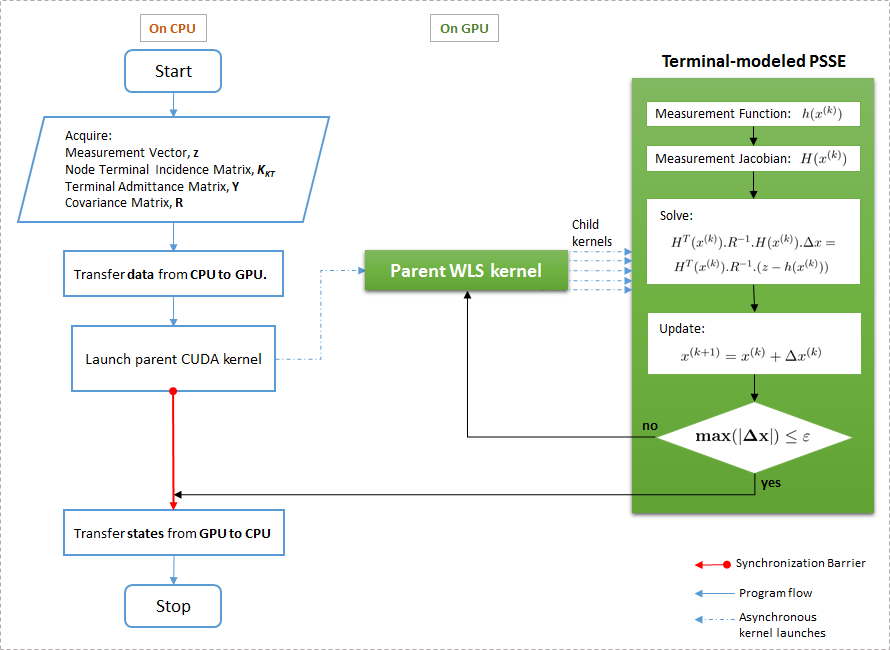
\includegraphics[scale=0.85]{cudasewdp}
	\caption{Ported SE using CUDA, with Dynamic Parallelism}
	\label{fig:cudasewdp}
\end{figure}


\subsection{Limitations of SE using Dynamic Parallelism}
While elimination of PCIe data transfers from GPU to CPU can be beneficial, the support for Dynamic Parallelism as of now is limited from hardware as well as software standpoints. The limitations encountered during the implementation are listed below:
\begin{enumerate}
	\item In comparison to a CPU core, CUDA cores have smaller cache and lower clock frequencies. Unlike CPUs, they do not have sophisticated branch prediction or speculative execution.
	\item Lack of support for C++ Standard Template Library makes development of custom device memory manager cumbersome. Due to this, the numerous memory allocations have to be made manually for every step of the computation.
	\item As of CUDA 9.1, cuBLAS can be called from device code. However, the support for cuSOLVER in device code is missing. The solution of a linear system with 1 right-hand-side can be computed using cuBLAS as follows:
		\begin{enumerate}
			\item LU Decomposition of the coefficients:  \inlinecode{C}{cublas<t>getrfBatched()}
			\item Inverse Computation of the LU decomposed matrix:  \inlinecode{C}{cublas<t>getriBatched()}
			\item GeMV dot product: \inlinecode{C}{cublas<t>gemv()} (Solution)
		\end{enumerate}
	Although the functionality of cuSOLVER can be substituted with the aforementioned cuBLAS function calls, it comes at the cost of performance degradation. This is because these functions are intended to be used for an array of matrices of relatively small sizes where the launch overhead is a significant factor~\cite{cuBLAS}. The following graph in Figure \ref{fig:dpdegrad} shows the comparison between execution times for obtaining the solution of a linear system using the given two approaches:
\end{enumerate}

\begin{figure}[H]
	\centering
	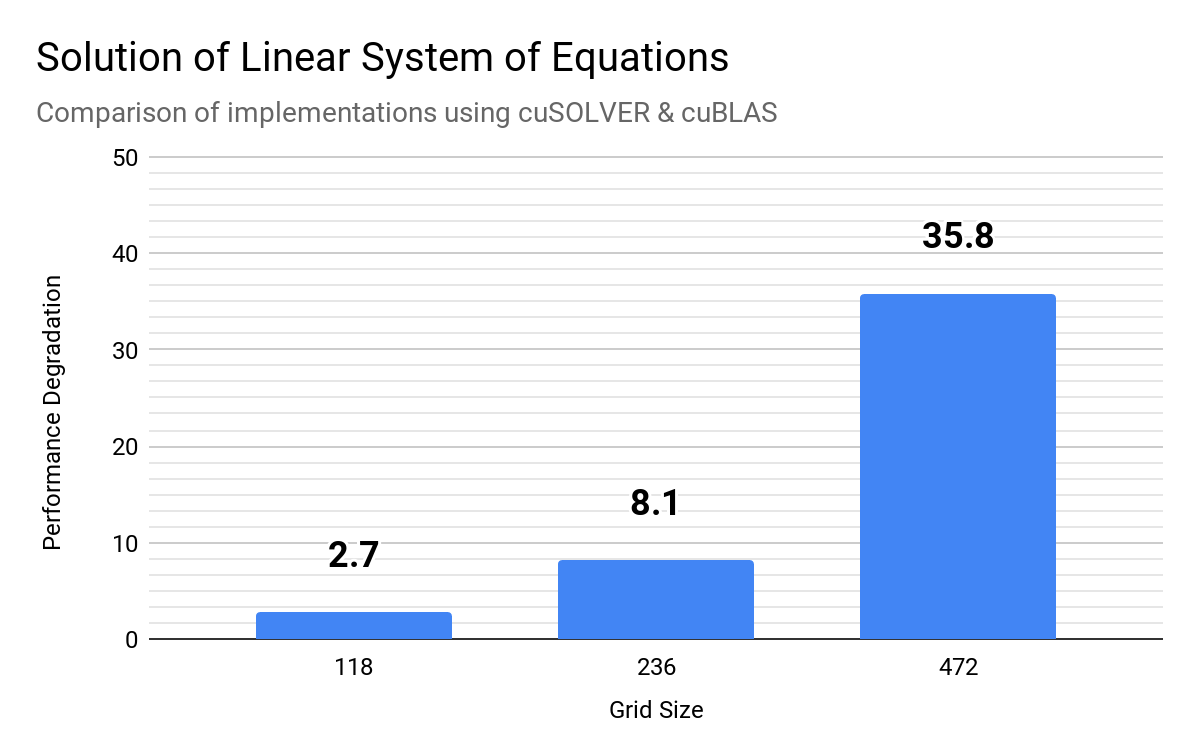
\includegraphics[scale=0.4]{dpdegrad}
	\caption{Comparison of solution times}
	\subcaption*{It is calculated as $t_{cuBLAS}:t_{cuSOLVER}$. Used GPU: Tesla V100}
	\label{fig:dpdegrad}
\end{figure}
It is therefore estimated that despite Dynamic Parallelism is an attractive option, the aforementioned limitations can collectively further give rise to considerable performance degradation. Hence, taking them into account, only the implementation without Dynamic Parallelism is used for evaluation purposes.

\subsection{FP32 and FP64 Variants}
In Section~\ref{sec:hardware}, it can be observed that there exists a remarkable discrepancy between FP32 and FP64 peak throughputs. On GTX 1070, in the time required for 32 FP32 operations, only 1 FP64 operation is performed. However, on scientific-computing GPUs like Tesla V100 or Titan V, the ratio for FP32:FP64 throughputs is 2:1. In either case, due to the considerably higher peak arithmetic throughputs for FP32, better performances can be achieved using single-precision operations. Therefore, the accelerated SE application described in Section \ref{sec:accse} is made to support the two precisions. \\
As in a typical C/C++ program, the FP32 and FP64 values are represented using data-types float and double respectively. On the other hand, the relevant complex numbers with FP32 or FP64 components can be represented using cuComplex or cuDoubleComplex structs respectively. C++ templates may be used to prepare generic kernels which can be casted into their specific types during compilation.\\
The predetermined constant $\epsilon$ must be chosen differently for both precision levels due to potential rounding errors described in Section \ref{sec:spvsdp}.

\section{Porting Techniques}\label{sec:portimpl}
Upon a thorough inspection of the serial SE algorithm, numerous operations are found which are either of arithmetic or linear algebraic nature or involve helper-operations like slicing of matrices using given indices. The following table \ref{table:cudasolutions} details the operations that require porting to CUDA alongside their corresponding solutions:
{\renewcommand{\arraystretch}{1.3}%
\begin{table}[H]
	\begin{tabular}{|
			>{\columncolor[HTML]{C0C0C0}}l |l|
			>{\columncolor[HTML]{C0C0C0}}l |l|}
		\hline
		{\color[HTML]{000000} GeMM/GeMV}             & {\color[HTML]{000000} cuBLAS}   & {\color[HTML]{000000} Slicing}                    & CUDA kernel \\ \hline
		{\color[HTML]{000000} Max Reduction}         & {\color[HTML]{000000} cuBLAS}   & {\color[HTML]{000000} Concatenation}              & CUDA kernel \\ \hline
		{\color[HTML]{000000} Transpose}             & {\color[HTML]{000000} cuBLAS}   & {\color[HTML]{000000} Diagonal Flattening}        & CUDA kernel \\ \hline
		{\color[HTML]{000000} Linear Algebra Solver} & {\color[HTML]{000000} cuSOLVER} & {\color[HTML]{000000} Identity matrix generation} & CUDA kernel \\ \hline
		\cellcolor[HTML]{656565}                     & \cellcolor[HTML]{656565}        & Map Operations                                    & CUDA kernel \\ \hline
		\cellcolor[HTML]{656565}                     & \cellcolor[HTML]{656565}        & ASMD                                              & CUDA kernel \\ \hline
	\end{tabular}
	\caption{CUDA solutions for necessary matrix operations}
	\label{table:cudasolutions}
\end{table}}

Some of these operations are used exclusively for data preparation. The WLS loop iterations make frequent use of GeMM, ASMD, slicing and linear algebra solver operations. As seen in the table above, most of these operations can be implemented using existing optimized CUDA libraries while the remaining functions are ported using user-defined CUDA kernels.

\subsection{Porting using cuBLAS \& cuSOLVER}
cuBLAS and cuSOLVER libraries are extensively used throughout the computation for calculating matrix-matrix/matrix-vector dot products and solution of linear system of equations respectively. However, in order to maintain compatibility with FORTRAN applications, these libraries are constructed assuming column-major storage of vectors and matrices as opposed to C/C++ which assumes row-major storage. Due to column-major access, a matrix supplied by the system is seen as its transpose by the library and vice versa. This necessitates different than usual configuration of the input matrices.\\
Some of the operations implemented using these 2 libraries are described below:

\subsubsection{GeMM Dot Product}
In order to compute the dot product of 2 matrices $\textbf{\textit{A}}$ and $\textbf{\textit{B}}$, the correct configuration of matrices can be ascertained using the following property of matrix transpose:
\begin{equation}\label{eq:transposeproperty}
(\textbf{\textit{AB}})^{T} = \textbf{\textit{B}}^{T}\textbf{\textit{A}}^{T}
\end{equation}
Based on equation~\ref{eq:transposeproperty}, 
\begin{enumerate}
	\item The matrices are supplied by the user (in reverse order).
	\item The entered matrices are seen as their transposes by the library, i.e. \\$\textbf{\textit{B}} \Rightarrow \textbf{\textit{B}}^{T}$; $\textbf{\textit{A}} \Rightarrow \textbf{\textit{A}}^{T}$ 
	\item The library produces the dot product of the transposes, i.e. $\textbf{\textit{B}}^{T}\textbf{\textit{A}}^{T} $
	\item From equation~\ref{eq:transposeproperty}, result from 3 is equal to the transpose of the dot products of matrices in original order. 
	\item The transpose of the dot product is however seen as the dot product by the user. 
\end{enumerate}

\begin{figure}[H]
	\centering
	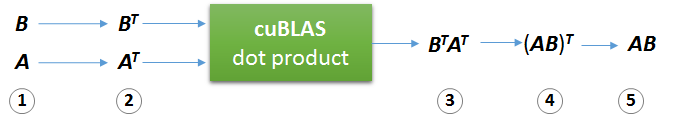
\includegraphics[scale=0.85]{cublasdot}
	\caption{Calculation of dot product $\textbf{\textit{AB}}$ using cuBLAS}
	\subcaption*{The column-major storage assumption of the library necessitates configurations based on properties of matrix transposes.}
	\label{fig:cublasdot}
\end{figure}

\subsubsection{Max Reduction}
This operation is used to extract the maximum residual error at the end of every WLS iteration. It can be implemented using a CUDA kernel that performs reduction or by using cuBLAS API. The steps to extract maximum value from a given vector using cuBLAS are as follows:
\begin{enumerate}
	\item In cuBLAS, \inlinecode{C}{cublasI<t>amax()} returns the index of the element with maximum magnitude in a given vector. Let the index be \inlinecode{C}{max_index}.
	\item The index returned is based on FORTRAN indexing. It must be therefore decremented by 1 to get C-based index, i.e. \inlinecode{C}{max_index--}
	\item The value at the given index is then retrieved as follows:\\
		\inlinecode{C}{float max;}\\
		\inlinecode{C}{cudaMemcpyAsync(&max, devArry + max_index, sizeof(float), cudaMemcpyDeviceToHost, stream);}
\end{enumerate}


\subsubsection{Linear Algebra Solver}
In order to compute the solution of a dense linear system with one or more right hand sides using cuSOLVER, the following function calls must be made:
\begin{enumerate}
	\item \inlinecode{C}{cusolverDn<t>getrf()} - This function computes LU factorization of a matrix $\textbf{\textit{A}}$.
	\item \inlinecode{C}{cusolverDn<t>getrs()} - This function computes the solution using LU-factorized matrix $\textbf{\textit{A}}$ of and its right-hand-side matrix $\textbf{\textit{B}}$. The solution is returned by overwriting matrix $\textbf{\textit{B}}$.
\end{enumerate}


\subsection{User-defined CUDA Kernels}
For those operations that cannot be implemented using the existing official libraries, CUDA kernels can be written using CUDA C. The kernels are written to execute on matrices of arbitrary dimensions, i.e. the matrix dimensions may or may not be a multiple of 32. The grid and block size must be chosen appropriately based on the input matrices. A block size of \inlinecode{C}{dim3(32, 32, 1)} is frequently used. However, for a row matrix, the dimension can be be changed to \inlinecode{C}{dim3(1024, 1, 1)}. Such kernel configurations are necessary to prevent launch of unnecessary GPU threads.
Some of the important kernels written for this implementation are described below:

\subsubsection{Map Operations}
These operations include simple elementwise mapping of values in a given matrix. For example, calculating sine, cosine or absolute values of given floating point numbers as shown in code sample~\ref{code:mapOperations}. The following example kernel is used on a matrix with values of double datatype and computes its sine, cosine or absolute values based on the \inlinecode{C}{operationChoice} variable. This variable is a fixed value decided before kernel-launch and therefore does not cause warp-divergence.
\lstset{aboveskip=10pt,belowskip=10pt} % space above and below lstlistings
\begin{lstlisting}[language=C, caption={CUDA kernel for map operations: sin, cosine or absolute values of given matrix}, captionpos=b, label={code:mapOperations}]
__global__ void matrixElementWiseSinOrCosOrAbs(double *idata, double *odata,
											   int width, int height, int operationChoice)
{
	// Compute thread 2D global coordinates
	int global_2D_x = blockDim.x * blockIdx.x + threadIdx.x;
	int global_2D_y = blockDim.y * blockIdx.y + threadIdx.y;
	
	// Processing only those threads which are within matrix dimensions
	if (global_2D_x < width && global_2D_y < height)
	{
		// Calculating global 1D index for accessing the matrix in row-major fashion
		int global_1D_index = global_2D_x + global_2D_y * width;
		
		// Depending on the operation choice, it either adds or subtracts
		if (operationChoice == 0) // Sin operation
			odata[global_1D_index] = sin(idata[global_1D_index]);
		else if (operationChoice == 1) // Cos operation
			odata[global_1D_index] = cos(idata[global_1D_index]);
		else if (operationChoice == 2) // Abs operation
			odata[global_1D_index] = fabs(idata[global_1D_index]);
	}
}
\end{lstlisting}

\subsubsection{Slicing}
Since the serial algorithm makes extensive use of indexing for efficiency, slicing operation from MATLAB is ported to CUDA as well. Although significant effort has been made to prevent warp divergence, operations like slicing are nevertheless affected. In the kernel code~\ref{code:matslice}, the CUDA threads that lie within the specified x-axis and y-axis bounds shall execute the code within the conditional block whereas the others will be masked off. In addition to that, since the kernel is executed on matrices of variable sizes, the achieved occupancy and branch efficiency of the kernel varies widely.
\lstset{aboveskip=10pt,belowskip=10pt} % space above and below lstlistings
\begin{lstlisting}[language=C, caption={CUDA kernel for matrix slicing}, captionpos=b, label={code:matslice}]
__global__ void slice(const double *input,
						   double *output,
						   const int row_start,
						   const int row_end,
						   const int column_start,
						   const int column_end,
						   const int input_matrix_width,
						   const int output_matrix_width)
{
	// Compute thread 2D global coordinates
	int global_index_X = blockIdx.x * blockDim.x + threadIdx.x;
	int global_index_Y = blockIdx.y * blockDim.y + threadIdx.y;
	
	// Refer to the global coordinates in terms of row and column for ease
	int row = global_index_Y;
	int column = global_index_X;
	
	// Checking if the thread coordinates exist within specified bounds.
	if (row >= row_start && row < row_end && 
	column >= column_start && column < column_end) 
	{
		output[(global_index_X - column_start)
			+ (global_index_Y - row_start) * output_matrix_width]
				= input[global_index_X + global_index_Y * input_matrix_width];
	}
}
\end{lstlisting}


\subsubsection{Matrix Concatenation}
One of the most frequent uses of concatenation is the preparation of the measurement function matrix $\textit{\textbf{h}}(\textit{\textbf{x}})$ and Jacobian $\textit{\textbf{H}}(\textit{\textbf{x}})$. Since such matrix-stacking operation is not supported by existing libraries, a CUDA kernel is written to achieve this functionality. This kernel allows horizontal as well as vertical stacking of matrices and the choice is made before launching the kernel. The following kernel code~\ref{code:matconcat} is launched twice to fill the target matrix with elements from the source matrices.
\lstset{aboveskip=10pt,belowskip=10pt} % space above and below lstlistings
\begin{lstlisting}[language=C, caption={CUDA kernel for matrix concatenation}, captionpos=b, label={code:matconcat}]
/*
This kernel handles matrix concatenation (horizontal or vertical) operations.

operationChoice:
0 = Horizontal concatenation
1 = Vertical concatenation
*/
__global__ void matrixConcatenateDouble(double *idata1, double *idata2, double *odata, 
										int width, int height, 
										int width1, int height1, 
										int width2, int height2, 
										int operationChoice, int isFirstMatrix)
{
	// Calculate global 2D coordinates
	int global_2D_x = blockDim.x * blockIdx.x + threadIdx.x;
	int global_2D_y = blockDim.y * blockIdx.y + threadIdx.y;
	
	// The first launch has isFirstMatrix=1 to extract elements from first matrix 
	if (isFirstMatrix) {
		if (global_2D_x < width1 && global_2D_y < height1) {
			int global_1D_index_source = global_2D_x + global_2D_y * width1;
			int global_1D_index_target = global_2D_x + global_2D_y * width;
			// Storing the first matrix's elements into the concatenated matrix
			odata[global_1D_index_target] = idata1[global_1D_index_source];
		}
	}
	// The second launch has isFirstMatrix=0 to extract elements from second matrix 
	else if (!isFirstMatrix) {
		if (global_2D_x < width2 && global_2D_y < height2) {
			int _1D_index_source, offset_1D_index_target;
			if (operationChoice == 0) {
				// Computing 1D index with x-offset=width1
				_1D_index_source = (global_2D_x)+global_2D_y * width2;
				offset_1D_index_target = (global_2D_x + width1) + global_2D_y * width;
			}
			else if (operationChoice == 1) {
				// Computing 1D index with x-offset=width1
				_1D_index_source = global_2D_x + global_2D_y * width2;
				offset_1D_index_target = global_2D_x + (global_2D_y + height1) * width;
			}
			odata[offset_1D_index_target] = idata2[_1D_index_source];
		}
	}
}
\end{lstlisting}

Apart from these, others include kernels for matrix element-wise ASMD, identity matrix generators, real or imaginary value extractions and diagonal-flattening of a given row or column matrix.

\section{Class Diagram of the CUDA Application}\label{sec:classdiagram}
The structure of the implemented CUDA-accelerated SE application is explained below:
\begin{itemize}
	\item DataImporter\\It consists of functions that load the matrices from given CSV files into the device memory. This may be extended to acquire data from other sources. It is also capable of partitioning acquired data for sectors based on the grid-sectorization configuration file (discussed later in Section ).
	\item CUDA\_Kernels\\It consists of user-defined kernels that can be used for both floating point as well as complex values.
	\item MemoryPool\\It consists of map of device allocation pointers or MAs (discussed in Section \ref{dmmse}).
	\item DeviceMemoryManager\\It consists of a collection of Memory Pools and is responsible for creating new MAs as well as recycling them.
	\item CudaFunctions\\This is an abstract class that consists of wrappers written to simplify calls to CUDA libraries as well as kernel launches. There exists two classes that inherit from this parent class and are specialized in FP32 and FP64 computations.
	\item StateEstimator\\It consists of the all the steps necessary to perform SE. It accepts data from DataImporter as input and applies SE algorithm to compute the state vector.
\end{itemize}
\begin{figure}[H]
	\centering
	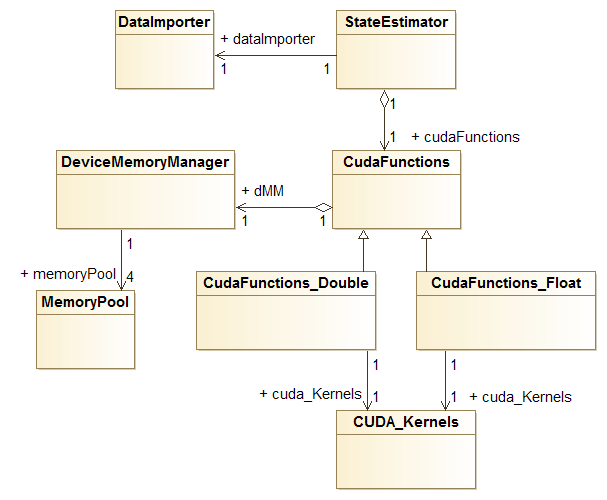
\includegraphics[scale=0.7]{cudacdse}
	\caption{Class Diagram of the application}
	\label{fig:cudacdse}
\end{figure}

\section{Integration of GPU-accelerated SE module in Decentralized Power Systems}\label{sec:integrationimpl}
Section \ref{sec:accse} describes the implementation of GPU-based SE for an entire power system. Based on the discussion in Section~\ref{consync} the SE for each grid sector obtained can be efficiently computed through concurrencies on CPU and GPU. Assigning each sector to a CPU thread and a GPU stream as shown in the Figure~\ref{fig:threadtostream} below results in high resource utilization by keeping the GPU always busy. 
\begin{figure}[H]
	\centering
	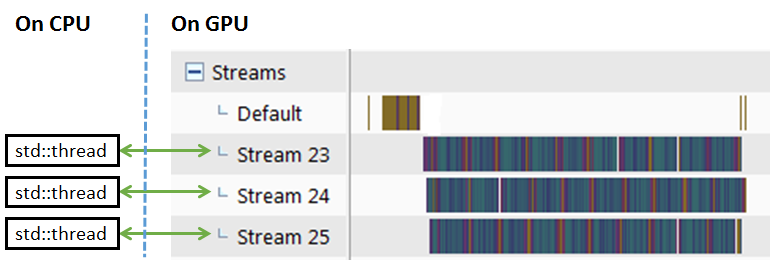
\includegraphics[scale=0.65]{threadtostream}
	\caption{Interaction of host threads with GPU Streams}
	\subcaption*{Each thread is assigned to a partition and is responsible for launching its computations independent of other threads.}
	\label{fig:threadtostream}
\end{figure}

The grid decentralization configuration is provided to the application using a properties file as shown below in Listing~\ref{code:decConf}. The file is parsed by the application before creating the partitions using slicing operation based on the data contained therein. The indices used within this file are 1-based in order to maintain easy portability of values from serial algorithm in MATLAB.
\lstset{aboveskip=10pt,belowskip=10pt} % space above and below lstlistings
\begin{lstlisting}[language=Python, caption={Grid decentralization configuration file}, captionpos=b, label={code:decConf}]
# Size of the grid
gridsize = 236

# Relative or absolute path to the dataset directory
path = SEdatasets\236

# It must match with the number of partition instances specified at the bottom
number_of_partitions = 2

# Partition Format: 
# partitionN={starting_bus, ending_bus, starting_terminal, ending_terminal} 
# Bus number starts from 1 (and NOT 0)
partition1 = {1, 118, 1, 372}
partition2 = {118, 236, 377, 750}
\end{lstlisting}
Figure~\ref{fig:dSEcuda} shows the flowchart illustrating the integration of GPU-accelerated SE module for decentralized power systems. After the individual state vectors are computed, they are subjected to a merger (described earlier in Section~\ref{merg}). In addition to that, in realistic situations, the resultant state vector is fed as the initialization instead of starting again with random data. This further helps in reducing convergence time.

\begin{figure}[H]
	\centering
	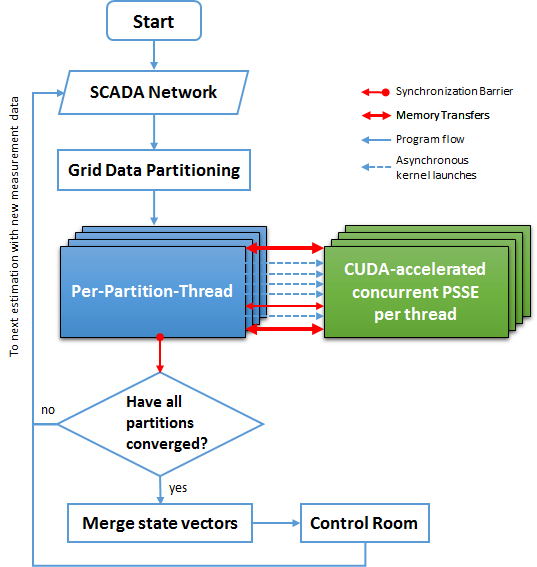
\includegraphics[scale=0.79]{dSEcuda}
	\caption{Decentralized SE using CUDA.}
	\label{fig:dSEcuda}
\end{figure}


\subfilebib % Makes bibliography available when compiling as subfile
\end{document}